\documentclass[11pt,a4paper]{report}

% Aberstwyth dissertation LaTeX Template
% Authors: Dr. Hannah Dee (hmd1@aber.ac.uk), Neil Taylor (nst@aber.ac.uk)
% This has been adapted from the Leeds Thesis template and the 
% Group Project template for Computer Science in Aberystywth University.
% 
% All comments and suggestions welcome.
%
% Template designed to be used with pdflatex: it may need alteration to
% run with a different LaTeX engine

% To build document on the unix command line, run four commands:
 
% pdflatex dissertation
% bibtex dissertation
% pdflatex dissertation
% pdflatex dissertation

% you will end up with dissertation.pdf 
\usepackage{mmp}

% the following packages are used for citations - You only need to include one. 
%
% Use the cite package if you are using the numeric style (e.g. IEEEannot). 
% Use the natbib package if you are using the author-date style (e.g. authordate2annot). 
% Only use one of these and comment out the other one. 
\usepackage{cite}
%\usepackage{natbib}

% Use the following to selectively exclude chapters
%\includeonly{chapter1}

\usepackage[T1]{fontenc}
\usepackage{graphicx}
\graphicspath{ {./images/} }
\usepackage{booktabs}
\usepackage[hypcap]{caption}
\usepackage{hyperref}
\usepackage{listings}
\lstset{%
	tabsize=2,
    basicstyle=\small,
    frame=tb
}
\usepackage{mdwlist}
\usepackage{pdfpages}
\hypersetup{
    colorlinks,
    linkcolor={red!70!black},
    citecolor={blue!70!black},
    urlcolor={blue!80!black}
}

\begin{document}

% all of the include directives below refer to tex files
% so \title{GOSH: Golang POSIX Shell}

% Your name
\author{Daniel Wakefield}

% Your email 
\authoremail{daw46@aber.ac.uk}

\degreeschemecode{G447} %e.g. G400 
\degreeschemetitle{Computer Science} % e.g. Computer Science
\degreetype{BSc}

\modulecode{CS39440} % i.e. CS39440, CC39440, CS39620
\moduletitle{Major Project} % i.e. Major Project or Minor Project

\date{20th March 2016} % i.e. the date of this version of the report

\status{Draft} % Use draft until you create the release version. Then, change this to Release.
\version{1.0}

%The title and name of your supervisor.
\supervisor{Prof. Dave Price} 

%The email for your supervisor. 
\supervisoremail{dap@aber.ac.uk}

\maketitle



 includes cover.tex - to change the content,
% edit the tex file

\pagenumbering{roman}

% This is the front page
\title{GOSH: Golang POSIX Shell}

% Your name
\author{Daniel Wakefield}

% Your email 
\authoremail{daw46@aber.ac.uk}

\degreeschemecode{G447} %e.g. G400 
\degreeschemetitle{Computer Science} % e.g. Computer Science
\degreetype{BSc}

\modulecode{CS39440} % i.e. CS39440, CC39440, CS39620
\moduletitle{Major Project} % i.e. Major Project or Minor Project

\date{20th March 2016} % i.e. the date of this version of the report

\status{Draft} % Use draft until you create the release version. Then, change this to Release.
\version{1.0}

%The title and name of your supervisor.
\supervisor{Prof. Dave Price} 

%The email for your supervisor. 
\supervisoremail{dap@aber.ac.uk}

\maketitle



                        

% Set up page numbering
\pagestyle{empty}

% declarations of originality 
\thispagestyle{empty}

%%%
%%% You must sign the declaration of originality. 
%%%
\begin{center}
    {\LARGE\bf Declaration of originality}
\end{center}

In signing below, I confirm that:

\begin{itemize}
\item{This submission is my own work, except where 
clearly indicated.}

\item{I understand that there are severe penalties for 
Unacceptable Academic Practice, which can lead to loss 
of marks or even the withholding of a degree.}
 
\item{I have read the regulations on Unacceptable Academic 
Practice from the University's Academic Quality and 
Records Office (AQRO) and the relevant sections of the 
current Student Handbook of the Department of 
Computer Science.}
 
\item{In submitting this work I understand and agree to 
abide by the University's regulations governing these issues.}
\end{itemize}

\vspace{2em}
Name ............................................................  \\

\vspace{1em}
Date ............................................................ \\

%%% 
%%% We would like to make a selection of final reports available to students that take 
%%% this module in future years. To enable us to do this, we require your consent. You 
%%% are not required that you do this, but if you do give your consent, then we will have 
%%% the option to select yours as one of a number of reports as examples for other 
%%% students. If you would like to give your consent, then please include the following 
%%% text and sign below. If you do not wish to give your consent, please remove this 
%%% from your report. 
%%%
\vspace{1em}
\begin{center}
    {\LARGE\bf Consent to share this work}
\end{center}

In signing below, I hereby agree to this dissertation being made available to other
students and academic staff of the Aberystwyth Computer Science Department.  

\vspace{2em}
Name ............................................................  \\

\vspace{1em}
Date ............................................................ \\


               

\thispagestyle{empty}

\begin{center}
    {\LARGE\bf Acknowledgements}
\end{center}

I am grateful to...

I'd like to thank...
 % Acknowledgements
\thispagestyle{empty}

\begin{center}
    {\LARGE\bf Abstract}
\end{center}
This project aims to create GOSH, a POSIX shell developed in a modern type and memory safe language. 
                 % Abstract

\pagenumbering{roman}
\pagestyle{fancy}
\fancyhead{}
\fancyfoot[C]{\thepage}
\renewcommand{\headrulewidth}{0 pt}
\renewcommand{\chaptermark}[1]{\markboth{#1}{}}

\tableofcontents   
\newpage
\listoffigures
\newpage 
\listoftables
\newpage

% Set up page numbering
\pagenumbering{arabic}

\setchapterheaderfooter

% include the chapters
\chapter{Background \& Objectives}

%The aim of this project is to implement a UNIX command line shell that conforms to the POSIX shell standard\cite{POSIX-SHELL-STANDARD}.

%A command line shell is the minimal interface between users and the operating system kernel and allows users to work with a relatively simple read-eval-print loop.

%This section should discuss your preparation for the project, including background reading, your analysis of the problem and the process or method you have followed to help structure your work.  It is likely that you will reuse part of your outline project specification, but at this point in the project you should have more to talk about. 

%\textbf{Note}: 

%\begin{itemize}
%   \item All of the sections and text in this example are for illustration purposes. The main Chapters are a good starting point, but the content and actual sections that you include are likely to be different.
%   \item Look at the document on the Structure of the Final Report for additional guidance. 
%\end {itemize}

This Chapter provides some background information concerning the project.
The first section explains the concepts and importance of a command line shell.
The second section shows the problems that are apparent in the currently available shells.
The third section describes some of the research I conducted prior to beginning the project.
The fourth section analyses the problem and sets the objectives for the thesis.
The final section describes the development process that was used throughout the project.


\section{Background}
A shell is the smallest possible interface between a user and the operating system kernel.
The kernel provides API functions that perform complex tasks like launching executables, connecting to the network and accessing files.
The Domain Specific Language(DSL) of the shell simplifies these interactions and allows the user to focus on the things they want to do.

As well as providing this interface almost all shells can be used to interpret stored commands known as batch files or shell scripts.
These group commands to avoid repetition and to automate common tasks
Shells range in their support of these but all modern shells have conditionals, variables and structures that make them powerful scripting languages.
Shell syntax has been influential in the design of other modern scripting languages such as Perl and PHP.

There are two families of shells, those descended from sh and csh known as traditional shells and those that have a largely incompatible syntax and/or behaviour, known as exotic shells.
Fish\cite{FISH}, es\cite{ES-SHELL} and oh\cite{OH-SHELL}, which happens to be written in Golang, are examples of exotic shells.

However this thesis will focus entirely on the traditional shells as they have been ingrained into everyday computer science since the first generation where developed at Bell Labs (See figure~\ref{fig:shell-history}).

The POSIX shell specification\cite{POSIX-SHELL-STANDARD} describes what a shell should provide and how it should operate to be compat
(See figure~\ref{fig:shell-history}),

dash is a POSIX compliant shell which lacks many features useful in an interactive context.
Bash adds things such as history control, line editing and arrays but also has a compatibility mode for POSIX scripts.
Zsh has many extra features but also has emulation modes for its major rivals though they are not 100\% compatible.
These are all examples of modern traditional shells from the simplest to most complex.
XXX

Every Linux distribution right down to the very smallest\cite{ALPINE-LINUX} include a shell of some form that complies with 
The Almquist Shell(ash) and the Debian Almquist Shell(dash) are minimal shells that implement the spec.
However the most widely used shell, the Bourne Again Shell(bash), implements an incompatible superset of the POSIX functionality.
It comes with a flag to switch off the additional features and enable POSIX compatibility and when the binary is symlinked to \verb!/bin/sh! this flag is implicitly set.

This spec was introduced 'ex post facto' and was based on the ksh88 shell which  brought together the features from csh and the syntax from the bourne shell.  

\begin{figure}[hp]
    \centering
    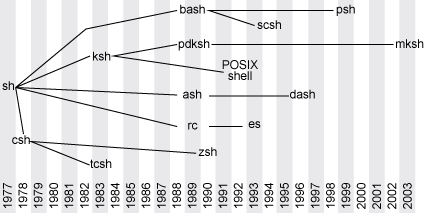
\includegraphics[width=0.8\textwidth]{xyz.png}
    \caption[Lineage of the main shells]{Lineage of the main shells\cite{SHELL-HISTORY}. Features where also incorporated across branches in many cases.}
    \label{fig:shell-history}
\end{figure}

\section{Motivations}
I have been using a shell ever I switched my operating system to Linux in 2009 it was my first introduction to useful programming.
I have been using one almost daily since, starting with bash and moving to zsh for the additional features and auto-complete.
During that time I have become a big fan of their terse syntax and quirks especially for codegolf\cite{CODE-GOLF}.

During my year in industry the ShellShock\cite{SHELLSHOCK-CVE,SHELLSHOCK-LWN,SHELLSHOCK-SYMANTEC} vulnerability was announced which drew my attention to the underlying technology.
I started examining the source code for bash once patches for shellshock and the subsequently discovered vulnerabilities were released.
The first thing I noticed was the huge amount of code that it consisted of (See table~\ref{tab:bash-loc}) and the low numbers of contributors.
While the OpenSSL codebase was in a worse state when the Heartbleed vulnerability broke earlier in the year that got two highly publicized forks attempting to modernize it (BoringSSL by Google\cite{BORINGSSL} and LibreSSL by The OpenBSD Foundation\cite{LIBRESSL}).
When nobody appeared to be attempting anything similar with bash I considered trying it myself.

A presentation on handwritten lexers\cite{PIKE-LEXING-VIDEO} given by Rob Pike, one of the creators of GoLang, intrigued me as everything seemed so simple and easy to follow. 
I had always assumed that implementing any language would have been extremely difficult as I'd only come across codebases in C that made heavy use of code generation.
Another presentation, given by Stephen Bourne, on the design of the original shell\cite{DESIGN-OF-SH-VIDEO} made clear that it was originally designed without the use of such tools.

Along with the book, Apprenticeship Patterns\cite{APPRENTICESHIP-PATTERNS} and the blog post, What Every CompSci Graduate Should Know\cite{EVERY-COMPSCI-GRAD}, these videos made implementing a shell seem like the type of thing that would push me to learn a great deal.
XXX

\begin{table}[hp]
\centering
\caption{Lines of code in bash's latest release (4.4-rc1)}
\label{tab:bash-loc}
\begin{tabular}{@{}lrrrr@{}}
\toprule
Language           & files & blank & comment & code   \\ \midrule
C                  & 252   & 20090 & 19392   & 102608 \\
HTML               & 3     & 3762  & 39      & 25942  \\
Bourne Shell       & 36    & 3330  & 3459    & 19857  \\
Teamcenter def     & 44    & 2567  & 1491    & 13014  \\
C/C++ Header       & 111   & 2719  & 3438    & 7286   \\
yacc               & 2     & 800   & 885     & 5096   \\
m4                 & 4     & 465   & 438     & 4656   \\
Perl               & 2     & 535   & 834     & 4229   \\
Bourne Again Shell & 24    & 196   & 249     & 786    \\
make               & 3     & 48    & 36      & 110    \\
Assembly           & 2     & 11    & 20      & 48     \\
awk                & 1     & 8     & 15      & 24     \\
sed                & 2     & 0     & 0       & 16     \\ \midrule
SUM:               & 486   & 34531 & 30296   & 183672 \\ \bottomrule
\end{tabular}
\end{table}


\section{Preparation}

XXX
To prepare for this project I started examining the source code for some of the modern traditional shells, including bash, dash and zsh.

To learn about compiler construction and language design I started studying from some of the courses available online that don't advocate using auto generation tools\cite{COMPILERS-COURSE,CRENSHAW}.
I also scanned through a book on lex\&yacc as both the are used in the bash source code and I wanted to be able to understand their use.

and reading books\cite{LEX-AND-YACC} and articles\cite{BUILD-INTERP,GOPHER-LEXING-BLOG} related to language design and compiler/interpretor construction. 


% ---------------------

% What was your background preparation for the project? What similar systems did you assess? What was your motivation and interest in this project? 

\section{Analysis} %========================================================

My original intention was to create a drop in replacement for bash but after examination of the source code for various shells it became clear that this was too ambitious.
The order of magnitude difference in lines of code between dash (Table~\ref{tab:dash-loc}) and bash (Table~\ref{tab:bash-loc}) suggests that the extra features present would add a huge amount of time to development and it would have been impossible to complete in the given time frame.
Despite this I want to develop the code so that after submission I can continue working on it to eventually reach my initial goal.

\begin{table}[hp]
\centering
\caption{Lines of code in dash's latest release (0.5.8)}
\label{tab:dash-loc}
\begin{tabular}{@{}lrrrr@{}}
\toprule
Language       & files & blank & comment & code  \\ \midrule
C              & 36    & 2120  & 2382    & 13153 \\
C/C++ Header   & 33    & 244   & 1049    & 1193  \\
make           & 2     & 100   & 38      & 655   \\
Bourne Shell   & 2     & 18    & 76      & 116   \\
Python         & 1     & 24    & 46      & 75    \\
Teamcenter def & 1     & 8     & 10      & 34    \\ \midrule
SUM:           & 75    & 2514  & 3601    & 15226 \\ \bottomrule
\end{tabular}
\end{table}

With that in mind I set out the high level objectives for the project.

\begin{itemize*}
    \item Create a POSIX\cite{POSIX-SHELL-STANDARD} compliant shell.
    \item Produce maintainable and easy to extend code.
    \item Provide a meaningful test suite consisting of both unit and integration tests.
    \item Become a more experienced Golang developer with a good portfolio piece.
\end{itemize*}

Some of these goals are vague and subjective but most importantly they don't make good assessment criteria.
To come up with some we need to look at a combination of what users expect from a shell and what the POSIX specification requires the shell to do.

The man page for the rc shell begins with:
\begin{lstlisting}
All of the following behave as expected:

date
cat /lib/news/build
who >user.names
who >>user.names
wc <file
echo [a-f]*.c
who | wc
who; date
vc *.c &
mk && v.out /*/bin/fb/*
rm -r junk || echo rm failed!
\end{lstlisting}

While this may not look like much it showcases a good portion of the features that most user's will need in their shell:
\begin{itemize*}
    \item Command execution with optional arguments.
    \item IO redirection to and from files.
    \item Filename and path globbing.
    \item Pipelining (IO redirections to concurrently running commands).
    \item Command chaining.
    \item Asynchronous commands.
    \item Conditional execution.
\end{itemize*}
The fact that these have been explicitly pointed out to work shows that these are considered the most important features.

Despite this I have decided to give development of IO redirection a low priority as it can be emulated through the use of pipes and utilities. \\
For example; output to a file \verb!foo | tee [--append] output_file! \\
and for input to a command \verb!cat input_file | foo!.\\
While these do not cover the full range of redirections, such as redirecting standard error, they will suffice to cover most situations and mean that development can be focused in other areas.

Along with these we can gather more required from the specification including:
\begin{itemize*}
    \item Variables, variable substitution and variable scoping.
    \item Shell functions.
    \item Command substitution / Subshells.
    \item Arithmetic substitution.
    \item Shebang support (e.g \#!/bin/foo).
    \item Control structures (if, while, until, for, case).
    \item Builtin commands.
    \item Word splitting.
    \item Job control.
\end{itemize*}

Most shells can run in two modes, interactive and non-interactive.
I decided that sticking to a shell that runs shell scripts well, ie non-interactive mode, would be preferable to having one with readline support, interactive mode, but that didn't work properly.
There is a Go implementation of readline that offers the required functionality\cite{GO-READLINE} so this would be a good extension if time allows.

My main analysis was based on the dash shell\cite{DASH} as it conforms to the POSIX shell standard\cite{POSIX-SHELL-STANDARD} while still having a reasonably small code base.
I also used the ash shell implementation included in busybox\cite{BUSYBOX} because of it's similarities.

The first thing you notice is that everything is built around three components, the Parser, the Lexer and a function called evaltree.
The lexer takes the raw string representation of the program and splits it into tokens.
These are feed, along with their values when appropriate, to the parser.
The parser intelligently groups these tokens into nodes representing high level structure inside the program.
This structure is known as an Abstract Syntax Tree(AST) and items in the tree are referred to as nodes.
The tree is then passed to the evaltree function which performs all of the actions contained within it.
It would also be possible to do away with the abstract syntax tree and interpret the code as it is parsed.

I decided against this for multiple reasons.
\begin{enumerate*}
	\item Separating the concerns of running a certain command from the parser means that a parse error will never leave execution in some undefined state.
	\item The tight coupling of the lexer, parser and evaluation would make it difficult to extend code in the future.
	\item All the texts I read encourage creating an AST for any future translations or optimizations. If at some point I decide I wanted to compile shell scripts to native binaries it would be impossible without one.
\end{enumerate*}

While these are the most important parts of the system as a whole I decided that starting with the arithmetic environment, '\verb!$(( ))!', would be a good idea.
This construct is sufficiently complex that it requires it own lexer and parser pair to keep the overall structure of the code simple but it is still just a glorified calculator.
Creating the lexer \& parser for this relatively simple language would give me experience working with them before I attempted to move onto the more complex main parser.


% ---------------------
These three components are some of the most important aspects of the code but they still will not operate correctly without other pieces of code being in place, such as the variable assignment and retrieval routines.

While this lexer and parser pair is quite complicated it should be possible to build so a single feature at a time is added to it.

Something that is notable is the use of global variables to hold parser and lexer state.

The first thing you notice about each shell is the general lack of comments, while the figures in table~\ref{tab:dash-loc} seem to show a good ratio of code:comments most of these are in fact repeated license headers in files.
This means it is both confusing and discouraging for newcomers to the codebase. 



Zmalloc

Linked Lists -> hash tables

Using the right data type where needed (nlflag should be a descriptive ENUM not int / tokpushback should be bool not int that is incr'ed, Be a function like hasNextToken)

Misleading names (CHKNL, why does it have to be short + it isnt checking newlines it is ingoring them)
% ---------------------

%Taking into account the problem and what you learned from the background work, what was your analysis of the problem? How did your analysis help to decompose the problem into the main tasks that you would undertake? Were there alternative approaches? Why did you choose one approach compared to the alternatives? 


%There should be a clear statement of the objectives of the work, which you will evaluate at the end of the work. 

%In most cases, the agreed objectives or requirements will be the result of a compromise between what would ideally have been produced and what was felt to be possible in the time available. A discussion of the process of arriving at the final list is usually appropriate.

\section{Process}
\label{sec:process}
%You need to describe briefly the life cycle model or research method that you used. You do not need to write about all of the different process models that you are aware of. Focus on the process model that you have used. It is possible that you needed to adapt an existing process model to suit your project; clearly identify what you used and how you adapted it for your needs.
The project was developed using a combination processes that included Feature Driven Development (FDD) and Test Driven Development (TDD).
This suited the project very well as I had a weekly meeting with my project supervisor which I set as the iteration duration.
Being able to announce that a certain feature or list of the features would be completed over the next week really drove me to work on them so I could prove I was making progress at each subsequent meeting.

Having a design that consisted of these feature sets and individual features was also hugely helpful as time progressed and we realised that the scope of the project would have to be reduced.

I was a single person team with only one meeting a week
TDD was used during the first few weeks as individual components where created but before they where connected.
It allowed me to show progress, prevent regressions and explicitly document the abilities of the code I was producing.

I switched to using an FDD approach once enough code had been produced that it could be linked together in a meaningful way.

FDD also lent itself well to this project as the overall model and feature list was provided to me in the form of the specification.
However the feature descriptions in the specification go into a large amount of extraneous implementation detail.
This detail could easily be ignored for the high level design and left to be incorporated into the feature design step.
Using the spec in this way allowed me to jump straight to implementing features once enough of the codebase was there to support them.

While I supplanted TDD with the more complete process of FDD they are complimentary techniques and often used together.
One of the steps of the feature build is code inspections and how this is done is decided on by the Team leader, called a Chief Programmer in FDD terminology.
It will often a combination of code review and testing, which in many modern development teams these tests is likely to be performed in a TDD manor.
I continued with unit tests and started adding integration tests once I switched process.
The confidence these tests gave allowed me to easily add and refactor features while ensuring that everything still worked as intended.  

One of the things I liked best about using this process was the constant feedback it gave me on the progression of the project.
If I became stuck on a certain feature I could always switch working branches and attempt to complete a smaller feature giving me time to think out the problems I had encountered with the other one.
Upon completion of a feature I always received a morale boost which really helped focus me on achieving the next goal in my list\cite{GETTING-REAL}.

During the development of my project, excluding the Easter holidays, I programmed with a friend who was working on their own project, which allowed us to keep each other motivated.
We often used each other for so called rubber duck debugging\cite{RUBBER-DUCK-DEBUG} which was very helpful. 
Comments made to each other on design and features usually provided insight into something we otherwise wouldn't have considered.


















%\addcontentsline{toc}{chapter}{Development Process}
\chapter{Design}

%You should concentrate on the more important aspects of the design. It is essential that an overview is presented before going into detail. As well as describing the design adopted it must also explain what other designs were considered and why they were rejected.

%The design should describe what you expected to do, and might also explain areas that you had to revise after some investigation.

%Typically, for an object-oriented design, the discussion will focus on the choice of objects and classes and the allocation of methods to classes. The use made of reusable components should be described and their source referenced. Particularly important decisions concerning data structures usually affect the architecture of a system and so should be described here.

%How much material you include on detailed design and implementation will depend very much on the nature of the project. It should not be padded out. Think about the significant aspects of your system. For example, describe the design of the user interface if it is a critical aspect of your system, or provide detail about methods and data structures that are not trivial. Do not spend time on long lists of trivial items and repetitive descriptions. If in doubt about what is appropriate, speak to your supervisor.
 
%You should also identify any support tools that you used. You should discuss your choice of implementation tools - programming language, compilers, database management system, program development environment, etc.

%Some example sub-sections may be as follows, but the specific sections are for you to define. 

\section{Language Choice}
As previously stated the language I chose for this project was Go.
This section aims to show why It was chosen over the other candidates I considered.

\subsection{Go}
Go, also known as Golang, is a statically typed, compiled, concurrent and garbage collected language heavily inspired by C for the general syntax, Limbo for it's use of Communicating Sequential Processes (CSP)\cite{HOARE-CSP} and Python for its emphasis on readability and an all inclusive standard library.
It is relatively modern, only released to the public in 2009, and was created to solve some of the problems experienced with the languages used at Google, namely C\verb!++!, Python and Java.
I began to learn it, through the Golang Challenge\cite{GOLANG-CHALLENGE},  during my industrial year after experiencing some of these problems with python myself.

The creators of the language are all well respected in the world of computing.
Rob Pike is known for Plan 9 and UTF8. 
Robert Griesemer for the Java hotspot VM
Ken Thompson for Unix, Plan 9 and B, the predecessor to C.
Their combined hatred of the complexity and compile times of C\verb!++! where the catalyst for Go's development.
They also saw it as an opportunity to improve upon the aspects of C that have been most problematic over the years including\cite{GO-DESIGN-EMAIL}.

\begin{itemize*}
	\item Optional braces around if statements (The cause of apples GOTO fail bug\cite{GOTOFAIL}).
	\item Pointer arithmetic.
    \item Unchecked array boundaries.
	\item Confusing side effects of post/pre increment and decrement. Go only allows the post version and only as a standalone expression.
	\item GOTO statements that can jump anywhere at any time.
    \item Overloaded return values used to indicate errors.
\end{itemize*}

The language also avoided style wars as it came with a tool, gofmt, that formats code 'the right way'.
This is just one of the ways in which Go is extremely opinionated.
Others include:
\begin{itemize*}
	\item Unused imports and variables are a compile time error.
    \item Variables names should be generally be short. The longer they are in scope the longer and more descriptive the name should be.
    \item The use of interface composition over polymorphism, generics and inheritance.
    \item One loop construct, the for loop. Use with a break statement to create a while or until loop.
\end{itemize*}

It also comes with a simple built in testing framework that encourages tests right from the start and a documentation generator emphasising that.

XXX
It also doesn't hurt that Go has been found that to be a great language to build components traditionally done with C, including things as complicated as a kernel subsystem\cite{GONET}.

Concurrency after moores law, cores increasing faster than ghz.

While this is the language I decided to go with in the end I did consider others.
The candidate list included C, C\verb!++!, Python and OCaml.

\subsection{C}
C is a fast, low level, general purpose compiled language that is extremely powerful.
Unfortunately this power comes at a cost.
Historically the readability of C code is low which means that maintaining and extending code is hard.
This would not a huge problem if I was only creating the project for the dissertation but I hope to continue development after submission.

I considered it as a candidate as many shells have already been written using it proving it is a suitable choice.
This could be considered both an advantage, the abundance of prior art, and a disadvantage, less room to find innovative solutions.

While I have used some C in the past and have read the seminal book, K\&R C, I would not consider myself experienced in its use, especially with the more modern aspects like compiler directives and function annotations.
This could have led to problems around having to learn parts of such a complex language while developing a large project.
Even though I did not end up using this language I spent lots of time reading the source code for dash, bash and busybox which are all written in C, therefore using it  may have helped in my context switches. 

One thing I was worried about was the minimal standard library that C implementations provide.
I assumed that I would be required to spend valuable development time creating standard functions and data structures.
However during my research I discovered that libraries such as GLib and qLibc are commonly used and provide most, if not all, of the things I am used to in the StdLib of Python.

I was also worried about introducing the classes of bugs common in C programs such as use after free, memory leaks, buffer under and over flows and format string attacks,


Something to note is that I discovered a library, libmill\cite{LIBMILL}, which provides functions and macros for Go like CSP.



\subsection{C++}


As with anything based in C, C\verb!++! may be considered the obvious step forward.
I have never used the language but have read the source code for a few projects written using it.
It has a fairly complete standard library and some of the memory management is abstracted behind constructor's and destructor's.
Despite this it is notoriously difficult and If the project where to use it it may be tied to one architecture and OS unless a lot of extra effort was put in.

\subsection{OCaml}
OCaml is a functional, garbage collected, compiled language.
It is a multi paradigm language that allows users to mix object oriented, imperative and functional styles.

I considered it as it is often said that ML languages are superior to imperative ones at creating compilers and interpretors. 
This is because construction and modification of tree structures, such as the abstract syntax tree required in interpretors, using pattern matching and algebraic data types is very idiomatic in these types of languages.

I chose to consider it over other functional languages as it had recently come to my attention when it was used to create the high profile language Hack at Facebook.
As well as this it has been used for the Haxe language, the MirageOS unikernel and many code analysis tools.
These are all complex systems that show that the performance and the bulitin parsing tools are up to tasks well above the complexity of a simple interpretor.

I however have no experience at all with OCaml and very little with ML languages in general.


\begin{figure}[hp]
    \centering
    \includegraphics[scale=0.7]{shell-design.png}
    \caption[Shell execution pipeline]{Shows how input is transformed along the way to being executed commands.}
    \label{fig:shell-flowchart}
\end{figure}


\section{High level design}
This section will describe the high level design of the shell and illustrate to a user with no knowledge of the internals of a shell how components interact with each other.

Figure~\ref{fig:shell-flowchart} is a visual guide to this though it should be noted that the flowchart is not totally representative of the system and is just here to show the progression of data.


\subsection{Input}
I chose to focus on the internals of the shell before making the input experience 'nicer'.
Input can be accepted in a variety of ways including reading from a pipe or file or through an interactive session.
After researching the complexities surrounding interactivity I decided it would have to be left out due to the time restrictions.
I plan to add interactivity in the future using the go-readline library\cite{GO-READLINE} and because of this some parts of the system where designed so that it could easily be plugged in.

The input text is important as it is used to construct the lexer which the parser requires to operate.

\subsection{Lexer}
The lexer I chose to write was a coroutine based non-deterministic finite automaton as described by rob pike in one of the presentations that inspired this project\cite{PIKE-LEXING-VIDEO}.
However as I came to learn this was not the ideal choice (See XXX).
There was also the choice of using a lexer generator such as ANTLR, but with Go being such a recent language these tools generally don't have support for it.
The Ragel tool is an exception to this.
In this section I will explain some of the lexing complexities that caused me to decide on a handwritten lexer over a generated one.

The lexer operates on the raw text a rune\footnote{Go has the concept of a rune which is a type alias of an int32 used to hold a unicode character.} at a time.
These runes are turned into a stream of normalized tokens, removing comments and whitespace.
In some cases newlines are also removed, e.g., when we are expecting some other terminating token such as the 'fi' following an 'if' block.
The lexer can also detect some errors that don't require deep knowledge of the language grammar such as unterminated strings and incomplete variable substitutions. 

However the POSIX spec is very lenient in most scenarios and many things that would be considered errors in other languages are ignored or resolved in some way.
An example of this is the variable symbol '\$'.
By itself or when followed by a invalid substitution character it becomes a literal character with no special meaning. This is very difficult to encode using a parsing expression grammar(PEG) or in Extended Backus–Naur Form(EBNF).

The lexer also handles other complex tasks such as command substitution lexing, which requires the creation of a sub parser to evaluate correctly and alias expansion.

Alias expansion means that the first word of any line should be checked against a list of expansions, if it matches the word is replaced by the expanded text and lexing begins again at the start of the line.
However as this example shows this can introduce a common compiler construction problems known as left recursion.
\begin{verbatim}
# Direct left recursion
$ alias foo='foo xyx'
$ foo

# Indirect left recursion
$ alias foo='bar'
$ alias bar='baz'
$ alias baz='foo'
$ foo
\end{verbatim}
Care must be taken to avoid this as it will cause an infinite loop breaking the lexer and code generators are usually stumped by this.
Gosh does not currently support aliases but structures have been put in place so adding support in the future will be possible.

\subsection{Parser}
The next step is using the Parser to check the semantic meaning of these Tokens and to use them to create the nodes for an AST.
This is also the point where any remaining syntax errors should be detected.

I chose to write a predictive recursive descent parser(RDP) and some of the reasons why are:
\begin{enumerate*}
	\item It is a simple, logical design and is relatively easy to implement by hand.
    \item It works with the class of grammar that the shell language has (
    LL(1) explained further in XXX)
    \item dash and zsh both use RDP's giving some prior art to draw from as well as proving it is a suitable construct for the task.
\end{enumerate*}

The second option I considered was using a parser generator.
Go includes an implementation of yacc, one of the most famous, in its toolchain.
The Bash shell even uses bison to generate its parser.
However I feared that using one would have taught me more about the tool than parsers in general, making debugging of the generated code more difficult 
Chet Ramey, the maintainer of bash has also stated if he was starting over he would write a recursive descent parser himself\cite{BASH-ARCH} instead of using a generator.
This eliminated a LALR parser as a candidate.

The last option was a packrat parser.
Like recursive descent, this is a top down parser but it supports backtracking and is guaranteed to parse any LL(x) or LR(x) grammar in linear time.
This technology is very interesting but as it is still very new compared to other techniques it had not seen wide adoption by language designers.
This leads to a lack of prior art and other material to study and is the reason I did not consider it as a candidate further.

\subsection{Nodes \& the AST}
The Abstract Syntax Tree (AST) returned from the parser can consist of any number of nodes each of which can contain further child trees.

Nodes in this tree satisfy an interface called Node, which contains a single method called Eval.
Each Node is a separate type that contains fields relevant to itself.
The types then satisfy this interface with code that knows how to perform the actions of that node and hand execution off to child nodes when appropriate.

As with any tree something has to be terminal.
There are three things that are considered terminal when returned from the parser and each is treated differently.

The NodeCommand is terminal since it returns an exit code, but it is also a valid AST.
This node handles execution of system utilities, builtins and user defined functions as well as the redirection of their input and output to the requested files, pipes or file descriptors.
This is known as a 'simple command' in the specification and is the building block for 'compound commands'.

The NodeEOF indicate that the input has been exhausted and the shell should return with the last exit code it received.
The main loop checks explicitly for it with a type check.
The layout of the parser means that nothing else can receive this as a valid node.

Finally there is 'nil' which is to be used as a signal to the interactive session.
It is also used in the NodeCaseList to indicate that the case contains no code.
XXX %This should be changed to a NOOPNode which NodeEOF can embed.

Go allowed me to express nodes in a clean way through the use of interfaces and structs.
This is a big change from how they are expressed in dash's C code.
There they consist of DEFINED constants, huge union structs and evaluation code in a single function with GOTO's and XXX

\subsection{Expansion}
While the diagram shows that only NodeCommands undergo expansion this is a slight lie to keep it simple.
The Arg structures contained in a NodeFor and a NodeCase are also expanded when required but they don't cause any command execution.

When evaluation hits a NodeCommand we know we are going to do either set some variables \verb!A=1 B=2! or run some sort of command, with optionally prepended assignments\verb!A=1 foo!.
In either case it is possible that a value exists that requires expansion e.g \verb!A="$X $(foo) $((3+4))" B=*.c!.

The expansion pipeline performs these expansions in order returning a list of strings as some of the expansions can result in multiple words.
These include:
\begin{description*}
	\item Tilde expansion \hfill \\
    	Turning the '\textasciitilde' character into the filepath of home or named directory's.
    	This expansion only occurs at certain positions in unquoted words.
    \item Subshell expansion \hfill \\
    	This expansion starts another evaluation loop with certain IO redirections so the output of the subshell can be placed as a string in its place.
	\item Arithmetic expansion \hfill \\
    	Arithmetic is sufficiently complicated that it requires a call to a separate lexer parser pair.
        This expansion calls the exposed Parse function and receives an integer in return which can be converted to a string.
    \item Variable Substitution \hfill \\
    	There are some complex variable replacements which can alter the contents, assign new values or even exit the shell with an error in some cases.
	\item Filepath globbing \hfill \\
    	Unquoted strings containing globbing meta characters are expanded to a list of files in the current directory that match the pattern.
        If no files match the pattern it is returned as a literal string.
\end{description*}

Bash and other modern shells extend these further to include brace expansion and process substitution.

\subsection{Execution}

XXX



\section{Arithmetic}
This section is about the arithmetic construct, the reasons why it requires a separate lexer-parser and how this pair differs from the one used for the general shell language.



















\section{Other relevant sections}
\chapter{Implementation}

%The implementation should look at any issues you encountered as you tried to implement your design. During the work, you might have found that elements of your design were unnecessary or overly complex; perhaps third party libraries were available that simplified some of the functions that you intended to implement. If things were easier in some areas, then how did you adapt your project to take account of your findings?

%It is more likely that things were more complex than you first thought. In particular, were there any problems or difficulties that you found during implementation that you had to address? Did such problems simply delay you or were they more significant? 

%You can conclude this section by reviewing the end of the implementation stage against the planned requirements. 

\section{Arithmetic Lexer \& Parser}
This was the first component that was created.
The fact that it stands alone and its only interactions are getting and setting variables made it the perfect starting point.
The lexer is simple as symbols are either digits, variable names --- which always start with a letter or underscore--- or identifiers which are special characters like '+'


Most of my research on was done during this stage which helped me decide on the type of parser I wanted to create

\subsection{Variables}
\subsection{Ternary Bug}

\section{Scope}

\subsection{Variables}
\subsection{User Functions}
\subsection{Aliases}

\section{Main Lexer}

\subsection{Strings}
\subsection{Variables}
\subsection{Subshells}
\subsection{Arithmetic}

\section{Main Parser, AST \& Nodes}

\subsection{Simple Command}
\subsection{Command}
\subsection{Pipeline}
\subsection{And Or}
\subsection{List}

\section{Expansion}

\subsection{Tilde}
\subsection{Substitutions}
\subsection{Globbing}
\subsection{Word Splitting}

\section{Builtin Commands}

\section{Circular Imports}





\chapter{Testing}

%Detailed descriptions of every test case are definitely not what is required here. What is important is to show that you adopted a sensible strategy that was, in principle, capable of testing the system adequately even if you did not have the time to test the system fully.

%Have you tested your system on "real users"? For example, if your system is supposed to solve a problem for a business, then it would be appropriate to present your approach to involve the users in the testing process and to record the results that you obtained. Depending on the level of detail, it is likely that you would put any detailed results in an appendix.

%the following sections indicate some areas you might include. Other sections may be more appropriate to your project. 

\section{Overall Approach to Testing}
This project took a detailed approach to testing due to the development process including TDD from the start and evolving into FDD when a more concrete product appeared.
This paid off multiple times catching bugs and regressions that occurred.

TDD was used throughout but focus switched from unit tests to integration tests as the complexity of test cases grew. 
The large size of the AST's produced for even simple statements (See~\ref{lst:if-ast-2}) meant that this swap saved significant time.

\section{Unit Tests}
Go comes with a builtin testing package as well as test runner tools to encourage testing from the beginning.
Tests can be placed in the same package as the code or they can use a special package ('X\_test' with X replaced by the package name) that only allows access to exported values.
This is a very simple way to ensure that any testing is blackbox and can help find places where package boundaries are too strict or weak.

Tests in Go are almost always table driven (See~\ref{lst:parser-unit-test} for an example).
This is the practice of testing with sets of inputs and comparing against the expected outputs.
The values used in these tests range from edge cases to common usage and are designed to stress the code.

\section{Integration Testing}
The integration testing for the project was done through sample shell scripts.
These exercised portions of the shell syntax and output a string during or after it.
A manually inspected each test files output to ensure that constructs where working as intended.




\section{Automated Testing}
Towards the end of the project I started using a continuous integration service called drone.io\footnote{My project's public page is available at \url{https://drone.io/github.com/Danwakefield/gosh}}.
Every time a commit was pushed to the github repository it would clone the code and run the both the unit and integration tests against the changes.
A notification email was sent if a build failed.

The system just ran the normal unit and integration tests however since this codebase can issue system calls it is safer to run these tests in a disposable container in case of a severe bug.  
CI systems also make it easy for contributors to see the status of the code and ensure that pull requests will not cause any regression.

\section{User Testing}
















\chapter{Evaluation}

%Examiners expect to find in your dissertation a section addressing such questions as:

%\begin{itemize}
%   \item Were the requirements correctly identified? 
%   \item Were the design decisions correct?
%   \item Could a more suitable set of tools have been chosen?
%   \item How well did the software meet the needs of those who were expecting to use it?
%   \item How well were any other project aims achieved?
%   \item If you were starting again, what would you do differently?
%\end{itemize}

%Such material is regarded as an important part of the dissertation; it should demonstrate that you are capable not only of carrying out a piece of work but also of thinking critically about how you did it and how you might have done it better. This is seen as an important part of an honours degree. 

%There will be good things and room for improvement with any project. As you write this section, identify and discuss the parts of the work that went well and also consider ways in which the work could be improved. 

%Review the discussion on the Evaluation section from the lectures. A recording is available on Blackboard. 

\section{Requirements}
As the requirements come mostly from the specification, it is hard 


\section{Design Decisions}
As has been noted in~\ref{sec:implementation}, a few of the design decisions where clearly wrong.

\subsection{Lexer}
The biggest problem was the design of the lexer being non re-entrant.
This prevented many syntax features from being completed and has left the shell in a non compliant state.
This things that where affected include:
\begin{itemize*}
	\item Embedded variables in both the arithmetic construct and complex substitutions.
    \item Complex substitutions that take multiple arguments.
    \item Alias expansions.
\end{itemize*}

While these could all have been accomplished with sublexers this would have been quite inefficient. 
Each lexer currently requires a complete copy of any remaining input text, a problem when parsing large scripts. 
Switching the lexers to take a Bytes.Buffer instead of a string for the input may help as slices\footnote{An array like structure that uses pointers into an actual array to reduce overhead.} could be taken from it.

Alias expansion is more difficult as there is lots of bookkeeping that 

\subsection{Package Layout}

\subsection{a}


\section{Suitability of tools}

\section{Other project aims}

\section{What would you do differently.}














% add any additional chapters here

\setemptyheader
\addcontentsline{toc}{chapter}{Appendices}
\chapter*{Appendices}
\pagebreak

% start the appendix - sets up different numbering
\fancypagestyle{plain}{%
%\fancyhf{} % clear all header and footer fields
\fancyhead[L]{\textsl{Appendix\ \thechapter}}
\fancyhead[R]{\textsl{\leftmark}}}

\appendix
\fancyhead[L]{\textsl{Appendix\ \thechapter}}
\fancyhead[R]{\textsl{\leftmark}}
\fancyhead[C]{}
\fancyfoot[C]{\thepage}
\renewcommand{\headrulewidth}{0.4pt}
\renewcommand{\chaptermark}[1]{\markboth{#1}{}}

\fancyhead[L]{\textsl{Appendix\ \thechapter}}
\fancyhead[R]{\textsl{\leftmark}}
\fancyfoot[C]{{\thepage} of \pageref{LastPage}}

% include any appendices here
\chapter{Third-Party Code and Libraries}

%If you have made use of any third party code or software libraries, i.e. any code that you have not designed and written yourself, then you must include this appendix. 

%As has been said in lectures, it is acceptable and likely that you will make use of third-party code and software libraries. The key requirement is that we understand what is your original work and what work is based on that of other people. 

%Therefore, you need to clearly state what you have used and where the original material can be found. Also, if you have made any changes to the original versions, you must explain what you have changed. 

%As an example, you might include a definition such as: 

%Apache POI library Ð The project has been used to read and write Microsoft Excel files (XLS) as part of the interaction with the clientÕs existing system for processing data. Version 3.10-FINAL was used. The library is open source and it is available from the Apache Software Foundation 
%. The library is released using the Apache License 
%. This library was used without modification. 

\lstinputlisting[caption={[fnmatch]fnmatch function. Originally from a gist published in 2010 \url{https://gist.github.com/kballard/272720}. See my fork of the code at \url{https://github.com/Danwakefield/fnmatch}. Forking was required as the code was created before Go V1 and I had to correct behaviour that had changed in that time. Attempted contact with the author failed\label{lst:fnmatch}}]{Appendix1/fnmatch.go}

XXX Move somewhere it counts. 
While Go has an fnmatch implementation available (import "path/filepath") is is hardcoded with settings for matching against file names. 
This would not work in the case list where globbing should not expand to a list of filenames but still requires matching against the same pattern syntax.
Therefore external code to perform this task was included.
LINK Github + gist.


\chapter{Ethics Submission}

This appendix includes a copy of the ethics submission for the project. After you have completed your Ethics submission, you will receive a PDF with a summary of the comments. That document should be embedded in this report, either as images, an embedded PDF or as copied text. The content should also include the Ethics Application Number that you receive. 
\chapter{Code Examples}

\begin{figure}[h]
\begin{lstlisting}[frame=tb]
type Node interface {
	Eval(*variables.Scope, *IOContainer) ExitStatus
}

type NodeIf struct {
	Condition Node
	Else      *NodeIf
	Body      Node
}

func (n NodeIf) Eval(scp *variables.Scope, ioc *IOContainer) ExitStatus {
	runBody := n.Condition.Eval(scp, ioc)
	if runBody == ExitSuccess {
		return n.Body.Eval(scp, ioc)
	}
	if n.Else != nil {
		return n.Else.Eval(scp, ioc)
	}
	return ExitSuccess
}     
\end{lstlisting}
\caption[The Node Interface]{The Node interface used in the AST. Also shows the NodeIf as an example of implementation. Interfaces are implicitly satisfied if the type has the required methods. \label{lst:node-interface}}
\end{figure}

\begin{figure}[h]
\begin{lstlisting}[frame=tb]
type NodeNoop struct{}

func (NodeNoop) Eval(*variables.Scope, *IOContainer) ExitStatus {
	return ExitSuccess 
}

type NodeEOF struct {
	NodeNoop
}
\end{lstlisting}
\caption[The EOF and No Op node]{The NodeEOF uses struct embedding to receive the methods of the NodeNoop.\label{lst:node-noop}}
\end{figure}


\begin{figure}[h]
\begin{lstlisting}[frame=tb]
func LeftShift(a, b int64) int64 {
	c := int64(math.Pow(2, float64(b)))
	if c == 0 {
		return a
	} else if c < 0 {
		panic("Negative Left Shift")
	}
	return a * c
}
func RightShift(a, b int64) int64 {
	c := int64(math.Pow(2, float64(b)))
	if c == 0 {
		return 0
	} else if c < 0 {
		panic("Negative Right Shift")
	}
	return a / c
}
\end{lstlisting}
\caption[Shift helper functions]{Go's compile time checks prevent using an int64 as an argument to a shift.\label{lst:arith-shift}}
\end{figure}

\begin{figure}[h]
\begin{lstlisting}[frame=tb]
switch currentCharacter:
case '<':
	switch l.next() {
	case '<':
		t = ArithLeftShift
		checkAssignmentOp = true
	case '=':
		t = ArithLessEqual
	default:
		t = ArithLessThan
		l.backup()
	}
}
if checkAssignmentOp {
	if l.hasNext('=') {
		t += ArithAssignDiff
	}
}
return t
\end{lstlisting}
\caption[Sample of Arithmetic Symbol Lexing]{Portion of the switch statement used to parse symbols. It shows how detection of the next token is possible using just 1 character of lookahead. '<', '<<', '<=' and '<<=' are all covered here.\label{lst:arith-symbol-lex}}
\end{figure}


\begin{figure}[h]
\begin{lstlisting}[frame=tb]
type ArithNode interface {
	nud(*Parser) int64
	led(int64, *Parser) int64
	lbp() int
}
\end{lstlisting}
\caption[ArithNode interface]{The interface required by the pratt parser for each node\cite{CROCKFORD-TDOP}. Differs from the examples by the addition of the parser arg to maintain state.
\label{lst:arith-node-interface}}
\end{figure}


\begin{figure}[h]
\begin{lstlisting}[frame=tb]
foofunc() {
	foo
}

true && {false; true} && echo "Reaches here"
echo "SUXXESS" | { tr X C && echo "Finished transform"} | tee /dev/null
\end{lstlisting}
\caption[Shell Command Grouping]{Shows command grouping being used in the definition of a function, a conditional list and in a pipe.
\label{lst:command-grouping}}
\end{figure}



\begin{figure}[h]
\lstinputlisting[language=c,caption={
[dash - evaltree]
The dispatch functions for evaluation of nodes in dash. Particularly confusing sections include the use of bit flags in the NAND/NOR/NSEMI case.
\label{lst:dash-evaltree}}]{Appendix3/evaltree.c}
\end{figure}



\begin{figure}[h]
\begin{lstlisting}[frame=tb]
if false; then
    $noop
else
    A="SUCCESS"
fi
\end{lstlisting}
\caption[Code for a simple if statement]{Shell code for an if statement. 'A' and 'noop' are previously set. The value of A is checked after the statement to ensure the code operated correctly.\label{lst:if-ast-1}}
\end{figure}

\begin{figure}[h]
\lstinputlisting[caption={
[AST for a simple if statement]
The AST produced for the code in~\ref{lst:if-ast-1}. 
\label{lst:if-ast-2}}]{Appendix3/AST-if.txt}
\end{figure}







\fancypagestyle{plain}{%
   \fancyhead{} %[C]{Annotated Bibliography}
   \fancyfoot[C]{{\thepage} of \pageref{LastPage}} % except the center
   \renewcommand{\headrulewidth}{0pt}
   \renewcommand{\footrulewidth}{0pt}
}

\setemptyheader

\nocite{*} % include everything from the bibliography, irrespective of whether it has been referenced.

% the following line is included so that the bibliography is also shown in the table of contents. There is the possibility that this is added to the previous page for the bibliography. To address this, a newline is added so that it appears on the first page for the bibliography. 
\addcontentsline{toc}{chapter}{Annotated Bibliography} % Adds References to contents page

%
% example of including an annotated bibliography. The current style is an author date one. If you want to change, comment out the line and uncomment the subsequent line. You should also modify the packages included at the top (see the notes earlier in the file) and then trash your aux files and re-run. 
%\bibliographystyle{authordate2annot}
\bibliographystyle{IEEEannot}
\renewcommand{\bibname}{Annotated Bibliography} 
\bibliography{References/references} % References file


\end{document}
